\section{Implementation}
\label{section:implementation}
\subsection{Mobile Player}
In this section the mobile player \gls{prefab} will be discussed. 
\gls{see} is supported on multiple platforms and with each platform having different requirements each platform needs to be divided.
Therefore, each platform gets its own player \gls{prefab}.
The mobile player prefab for the \gls{android} version of \gls{see} can be seen in figure \ref{fig:prefab}.

\begin{figure}[htb]
    \centering
    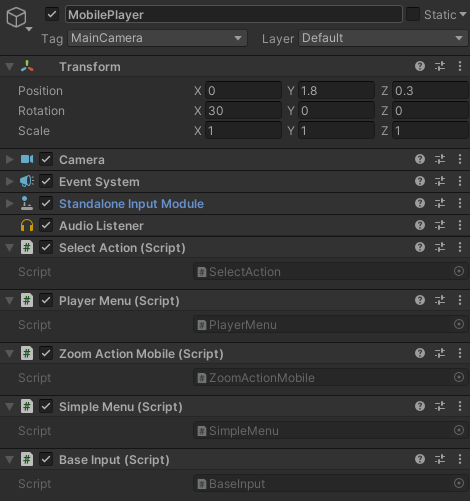
\includegraphics[width=0.8\textwidth]{Implementation/img/mobile_player.png}
    \caption{The mobile player \gls{prefab}}\label{fig:prefab}
\end{figure}

The \gls{prefab} consists of the basic parts provided by \gls{unity} \textit{Camera}, \textit{Event System}, \textit{Standalone Input Module} and \textit{Audio Listener}.
In addition to that the following custom scripts were added.
There is the \textit{SelectAction} and the \textit{ZoomActionMobile} script, which will both be discussed in section \ref{sec:player_actions}, and then there is the \textit{PLayerMenu} script, which creates the right menu based on the player type.
In this case the player type will be \enquote{mobile player} and the menu created (here \textit{SimpleMenu}) will be discussed in section \ref{sec:menu}.

\subsection{Player Movement}
After having creating a player, the player also has to be able to move.
Therefore, the \textit{MobilePlayerMovement} script got added.
The script handles the input by the joysticks seen in figure \ref{fig:joystick}.
To fulfill [R2.1] the player will be moved by using the left joystick and the player's perspective will be handled by the right joystick.

\begin{figure}[htb]
    \centering
    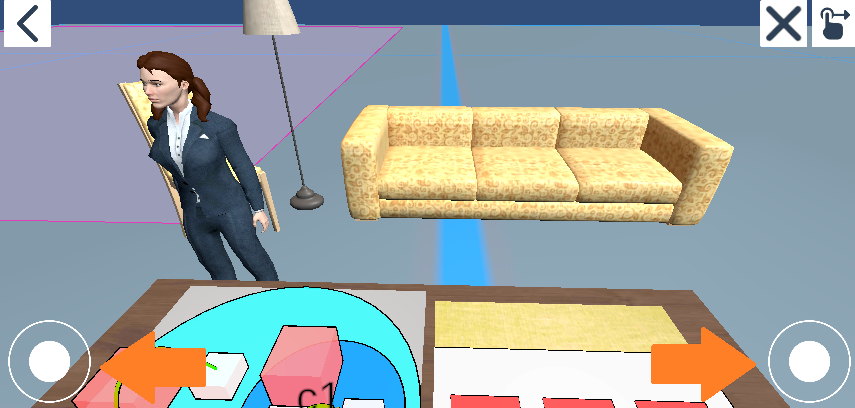
\includegraphics[width=1\textwidth]{Implementation/img/joysticks.png}
    \caption{The joysticks are for moving in the virtual room. The left joystick is for moving the player and the right one is for moving the player's perspective.}\label{fig:joystick}
\end{figure}

For the joystick \glspl{prefab} the \textit{Joystick Pack}\footnote{https://assetstore.unity.com/packages/tools/input-management/joystick-pack-107631\#description (last visited: 17.06.22, 15:21)} \gls{asset} is used.
It contains the design and basic logic for the joysticks.
A joystick returns a horizontal and a vertical value depending on how far the joystick is dragged into a direction.
The left joystick data can then be transformed into player movement as follows:
\begin{enumerate}
    \item Get the horizontal and vertical values from the joysticks
    \item Transform the values into a 3D vector
    \item Combine the values into a velocity vector
    \item Normalize the velocity vector for a smooth transition
    \item Transmit the velocity vector to the player position value
\end{enumerate}

The data of the right joystick shall move the player's perspective, which is implemented as a \gls{unity} camera.
The camera has a pitch angle and a yaw angle as illustrated in figure \ref{fig:camera}.
The angles of the camera will be adjusted with the input from the right joystick. 
For the angles of the player's perspective there is a range from 0° to 360° after reaching an end of this range the value will be transformed to the other end of the range.
In other words if the angle grows higher than 306° it starts an 0° again and if it gets lower than 0° it can go further down from 360°.
That way the player's perspective can move a full rotation.
\begin{figure}[htb]
    \centering
    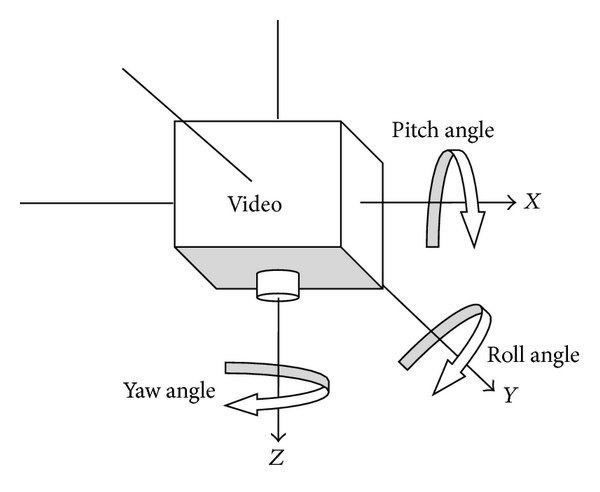
\includegraphics[width=1\textwidth]{Implementation/img/pitch_yaw.jpg}
    \caption{The angles of a camera by \cite{Zhang2014}}\label{fig:camera}
\end{figure}

\subsection{Mobile Menu}
\label{sec:menu}

The mobile menu is essential for the implementation since the input methods of a smartphone in an everyday usage are limited.
The desktop version uses many \glspl{shortcut}, which cannot be used in the mobile version.
These \glspl{shortcut} will replaced with buttons in the menu.

\begin{figure}[htb]
    \centering
    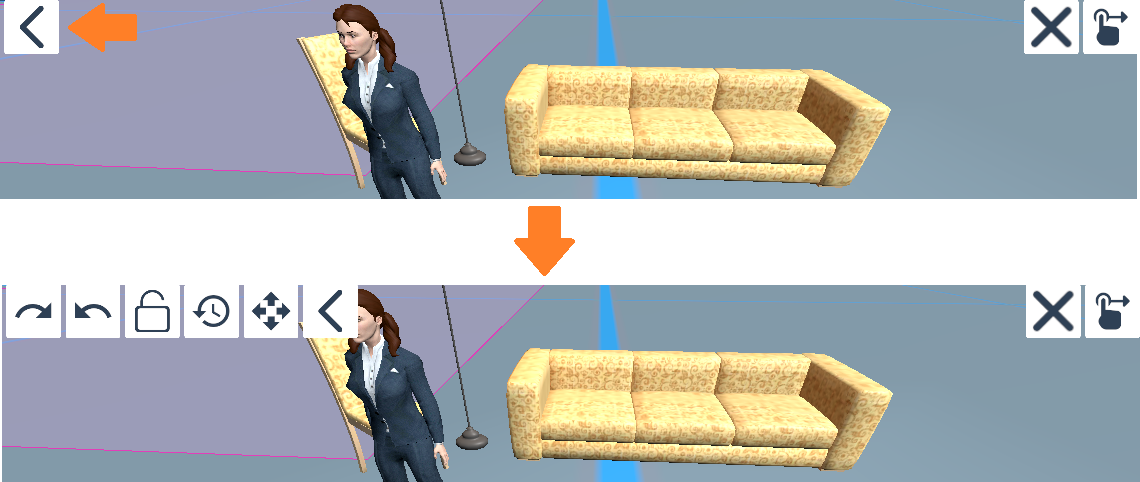
\includegraphics[width=1\textwidth]{Implementation/img/quickmenu.png}
    \caption{The \textit{quickbar} on the left top side of the mobile device. Pressing the button with an orange marked arrow will expand the menu.}\label{fig:quickmenu}
\end{figure}

The menu will be divided into to parts.
The first part, that was named \textit{quickbar} in section \ref{sec:interface}, will be responsible for all interactions that need to be available at all times.
The implemented \textit{quickbar} can be seen in figure \ref{fig:quickmenu}.
By pressing the button on the right end of the \textit{quickbar} the menu can be expanded and minimized to safe screen space when not needed.

The other part of the menu can be seen in figure \ref{fig:interaction_menu}.
The menu is placed on the right side of the screen, and it contains all the player interactions.

\begin{figure}[htb]
    \centering
    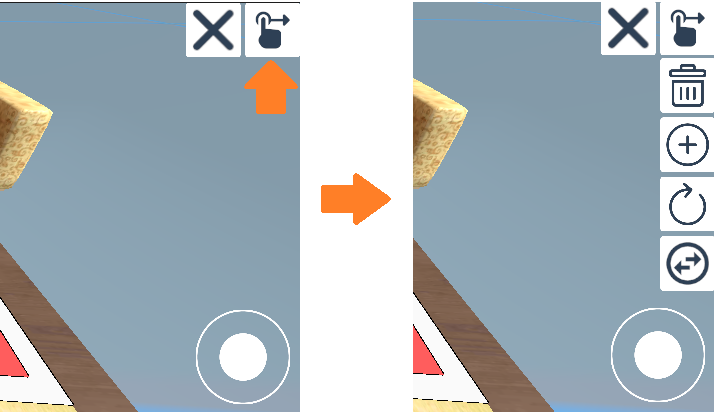
\includegraphics[width=1\textwidth]{Implementation/img/menu.png}
    \caption{The player interaction menu on the right top side of the mobile device. The button on the top right side indicate the active interaction mode. Pressing the same button also expands the menu.}\label{fig:interaction_menu}
\end{figure}

\subsection{Player Actions}
\label{sec:player_actions}